
 %参考《控制理论与应用》提供的LATEX模板  http://jcta.alljournals.ac.cn/uploadfile/cta_cn/20170419/kzllyy%20template20170419-2.9.zip
 % BHOSC   BUAAthesis  https://github.com/BHOSC/BUAAthesis/
 % 北航学报 http://bhxb.buaa.edu.cn/UserFiles/File/%E5%8C%97%E8%88%AA%E5%AD%A6%E6%8A%A5%E6%A8%A1%E6%9D%BF17.1.16(1).doc

 %%%% 五号字对应10.5pt,不知道这样设置对否?
\documentclass[10.5pt,twocolumn]{jbuaa}


%%画圆圈数字
\newcommand*\circled[1]{\tikz[baseline=(char.base)]{
            \node[shape=circle,draw,inner sep=1pt] (char) {#1};}}

%取消英文连词符
% \tolerance=1
% \emergencystretch=\maxdimen
% \hyphenpenalty=10000
% \hbadness=10000

\newcommand\mycolorRed[1]{{\color{red}#1}}
\newcommand\mycolorYellow[1]{{\color{yellow}#1}}
% \newcommand*\mycolorRed{\color{red}}

%%%????? 公式中字体的定义尺寸为 10 磅,上标/下标 68%,次下标/上标 42% ??????
\DeclareMathSizes{10.5}{10}{6.8}{4.2}
%%%% 本示例中带单位的数据采用的是siunitx来生成,好像默认与公式同样大小的字体,所以数字在正文中会小一些
%%%% 行文中普通数字大小为10.5pt,公式里或者用siunitx生成的数字则会是10pt,多少有点不协调。

%%%设置公式前后距离,差不多近似
\setlength{\abovedisplayskip}{2.5mm}
\setlength{\belowdisplayskip}{2.5mm}


\usepackage{tabu}
\usepackage{longtable}
\usepackage{makecell}
\usepackage[bookmarks=true,colorlinks,linkcolor=black]{hyperref}
\renewcommand\cellgape{\Gape[-3pt][-3pt]}


%%%%%%%%%%%%%%%%%%%%%%%%%%%%%%%%%%%%%%%%%%%%%%%%%%%%%%%%%%%%%%%%
%      文章正文
%%%%%%%%%%%%%%%%%%%%%%%%%%%%%%%%%%%%%%%%%%%%%%%%%%%%%%%%%%%%%%%%
\begin{document}
%%%%%%%%%%%%%%%%%%%%%%%%%%%%%%%%%%%%%%%%%%%%%%%%%%%%%%%%%%%%%%%%
% 标题,基金项目,作者,通信地址定义
%%%%%%%%%%%%%%%%%%%%%%%%%%%%%%%%%%%%%%%%%%%%%%%%%%%%%%%%%%%%%%%%
\title{
\vspace{1cm} \erhao\hei 智能电网中安全及隐私保护技术研究 \vspace{-0.2cm}
}


\author{
\sihao\fang 程潇 \makebox{$^{\text{1}}$}\\[0.1cm]
\liuhao (~~北京邮电大学~~网络空间安全学院,北京~~100876)
}

\date{}  % 这一行用来去掉默认的日期显示
%%%%%%%%%%%%%%%%%%%%%%%%%%%%%%%%%%%%%%%%%%%%%%%%%%%%%%%%%%%%%%%%
% 奇数页页眉
%%%%%%%%%%%%%%%%%%%%%%%%%%%%%%%%%%%%%%%%%%%%%%%%%%%%%%%%%%%%%%%%
\fancyhead[CO]{{\footnotesize 程潇:智能电网中安全及隐私保护技术研究}}            %请在这里写出第一作者以及论文题目
%%%%%%%%%%%%%%%%%%%%%%%%%%%%%%%%%%%%%%%%%%%%%%%%%%%%%%%%%%%%%%%%
%%%%%%%%%%%%%%%%%%%%%%%%%%%%%%%%%%%%%%%%%%%%%%%%%%%%%%%%%%%%%%%%
%  显示title,并设页码为空(按杂志社要求)
%%%%%%%%%%%%%%%%%%%%%%%%%%%%%%%%%%%%%%%%%%%%%%%%%%%%%%%%%%%%%%%%
%%%%%%%%%%%%%%%%%%%%%%%%%%%%%%%%%%%%%%%%%%%%%%%%%%%%%%%%%%%%%%%%
%      中文摘要
%%%%%%%%%%%%%%%%%%%%%%%%%%%%%%%%%%%%%%%%%%%%%%%%%%%%%%%%%%%%%%%%
\CKeyword{物联网; 智能电网; 安全架构; 用户隐私; 异常检测}
%\CLCNo{V221\makebox{$^{\scalebox{0.6}{\!+}}$}.3;TB553}
%\Dcode{A}
%\PaperNo{1001-5965 (XXXX) XX-XXXX-XX}

\twocolumn[
  \begin{@twocolumnfalse}
  \maketitle
%\positiontextbox{2.2cm}{2.9cm}{\wuhao http://bhxb.buaa.edu.cn \quad  jbuaa@buaa.edu.cn\\[0.3cm]
%\wuhao DOI: \ 10.13700/j.bh.1001-5965.****.****}
\begin{CAbstractJBUAA}
物联网作为国家五大新兴战略性产业之一,被称为继计算机、互联网后又一引领信息产业变革的技术。随着物联网技术的发展,加上人工智能技术的出现,一些传统行业开始与之结合,产生了像智能医疗、智能家居、智能电网等现代产业,但同时也带来了很多安全问题。智能电网(Smart Grid),作为电力系统与信息网络深度融合的产物,是一种典型的信息物理融合系统。智能电网系统的安全问题十分重要,而现在智能电网信息缺乏基本的隐私保护机制,从用电信息中中可以轻易获取用户个人信息,严重危害了用户隐私。

本文以物联网为背景,针对智能电网这个应用,提出了一个基于物联网安全架构模型的智能电网安全架构模型,本文从安全对象、安全架构和安全措施三个维度出发,总结出智能电网安全架构模型。此外,本文重点研究了智能电网中用户隐私的问题。本文的贡献如下:

1. 在对物联网安全参考模型的研究基础上,本文从安全对象、安全架构、安全措施三个维度归纳出智能电网安全
架构模型。从安全对象角度探讨了智能电网安全保护对象目标,从安全架构角度归纳了保证智能电网安全需要的技术手段,从
逻辑实施角度概括了智能电网需要用的到安全措施。

2. 通过本文提出的智能电网安全架构模型,本文以智能电网为研究对象,重点研究了智能电网保护用户隐私的问题。为了将智能电网保护用户隐私保护问题与异常检测方法关联起来,本文从对用户隐私定义的隐私维度出发,分析了对应在智能电网中的隐私维度,进而提出异常行为模式的定义。在异常行为模式的定义的基础上,论文研究并实现一种对智能电网异常检测的数据挖掘算法,该方法得到的自然排序也反应了该项数据的“异常程度”。

最后,本文利用公开智能电网数据集进行隐私挖掘和隐私保护的效果测试,设计了评估方法和实验,不过由于时间和人力的原因尚未进行具体实验。

\end{CAbstractJBUAA}
%%%%%%%%首页角注
%\positiontextbox{2.0cm}{25cm}{
%\noindent\rule{4cm}{.5pt}\\[0.5ex]%
%\hspace*{1em} \liuhao \linespread{0.8}\selectfont
%\parbox{\textwidth}{%
%\hei\makebox[\widthof{\makebox{*}收}][r]{收}稿日期: 2015-**-**; 录用日期: 2015-**-**; 网络出版时间:(此行信息已填) \\%
%\hei\makebox[\widthof{\makebox{*}收}][r]{网}络出版地址: (已填)\\
%\hei\makebox[\widthof{\makebox{*}收}][r]{基}金项目:国家自然科学基金(基金号~12345678);中国博士后科学基金(基金号~87654321)(注意:国家级基金放前,地方级放后)\\
%\hei\makebox[\widthof{\makebox{*}收}][r]{\makebox{*}通}信作者:E-mail:bhxb@buaa.edu.cn\\ \\
%\hei\makebox[\widthof{\makebox{*}收}][r]{引}用格式:(可不填)
%}}
  \end{@twocolumnfalse}
]


%%%%%%%%%%%%%%%%%%%%%%%%%%%%%%%%%%%%%%%%%%%%%%%%%%%%%%%%%%%%%%%%
%  正文由此开始-------------------------
%%%%%%%%%%%%%%%%%%%%%%%%%%%%%%%%%%%%%%%%%%%%%%%%%%%%%%%%%%%%%%%%
%%%%%%%%%%%%%%%%%%%%%%%%%%%%%%%%%%%%%%%%%%%%%%%%%%%%%%%%%%%%%%%%
%\wuhao
%  分栏开始

%%%%%!!!!!正文在第一页两栏分别合适位置插入 \enlargethispage{-3.3cm},给首页跨双栏脚注留空间,大小需要结合前面位置和高度手动设置!!!!!
%%%%%%%%%%%%%%%%%%%%%%%%%%%%%%%%%%%%%%%%%%%%%%%%%%%%%%%%%%%%%%%%

%《北京航空航天大学学报》严格执行科技出版的有关国家标准,如果作者返回的修改稿撰写不符合规范,特别是信息提供不完整,编辑部将联系作者要求答复、补正,这样常常费时费工也拖延文章出版。本文档简要介绍有关编辑出版规范和写作常识,请作者仔细阅读,认真执行,如有不明之处,欢迎来电咨询。您可以直接在本文档的基础上撰写稿件,使您撰写的文稿符合《北京航空航天大学学报》格式要求。\enlargethispage{-3.3cm}
%
%文章篇幅不限。
%
%\section{引言的说明}
%引言不编排节号,不插图列表。引言应说明课题的背景,引述该领域的国内外同行已经取得的进展,突出本研究工作的选题意义和创新点\citeBUAA{Harpold1979Shuttle,Yu2011Guidance}。内容不应与摘要和结论雷同\citeBUAA{Hu2015Steady}。在论述本文的研究意义时,应注意分寸,切忌使用“有很高学术价值”、“填补了国内外空白”、“首次发现”等不适之词;同时也注意不要使用客套话,如“才疏学浅”、“水平有限”、“恳求指教”之类的语言\citeBUAA{Laning1956Random,Zarchan2013Tactical,Zadeh1963Linear}。
%
%\section{题目、作者和单位}
%\enlargethispage{-3.3cm}
%题目应简洁、准确,能恰如其分地概括研究的范围和深度,避免使用希腊字母和上下标。英文题名中第一个单词首字母大写,其余小写(专有名词首字母大写)\citeBUAA{Weiss2005Adjoint,Zarchan1979Complete,Weiss2005Handover}。
%
%作者署名及署名排序应协商一致。姓名的英译采用汉语拼音,姓前名后,姓全大写,名首字母大写。如:ZHANG Ying(张颖),WANG Xilian(王锡联),ZHUGE Hua(诸葛华)。
%
%通讯作者一般为导师或课题负责人。
%
%单位应为论文首次投稿时的作者所在单位。单位的著录一般应到系一级,单位应著录全称,单位名称的英译应统一正确\citeBUAA{Lin1996ResearchAdjoint,Zou2001Adjoint}。

\section{绪论}
\subsection{研究的背景和意义}
1999 年,MIT(美国麻省理工学院)的 Kevin Ashton 教授首次提出物联网\citeBUAA{Ge2004IOT}(Internet of Things, IoT)的概念,说明了物联网的基本定义,即“万物皆可通过网络互联”。21世纪以来,伴随着全球经Gr2010securityCarpena2009Squences济的飞速发展,为了满足不断增长的能量需求,为了应对越发严峻的环境气候恶化,建立可靠、安全、高效、环保和用户友好的新型电力网络俨然已经成为一大研究热点。而智能电网(smart grid),作为电力网络与信息化深度融合的下的产物,被普遍认为是新一代电网技术解决方案。目前对于国内外、不同领域对智能电网的定义不一而足,但关键环节毫无例外地体现在信息技术与电力网络的结合。智能电网将现代信息、通信和控制技术深度应用于电力系统的发电、输电、变电、配电、用电和调度各个环节。从而,通过数字信息化,智能电网实现了信息流与电力流在电网内的一体化双向流动。最终,在充分满足用户的电力需求的同时,优化资源配置,保障安全运行,实现节能减排,提高经济效益。

在这样的大背景下,随着大数据的发展,物联网的内容隐私和安全问题变得尤其显著。物联网将万物互联,每时每刻都在产生着大量的数据,这些数据有一大部分由传感器网络通过用户的行为触发,故物联网网络产生的大数据反映了很多个人或团体的信息。
电力系统作为每个人每天必须接触使用的系统,当它演变为智能电网系统时,意味着每家每户的用电信息被数据化,这些数据通过信息挖掘可以暴露用户的个人习惯,生活习惯等。由此可见,信息安全传统的保证信息完整性,可用性,保密性已经不足以保证大数据时代信息安全。物联网环境下的信息安全是需要一个全盘的,全面的安全防护体系,这个体系是要贯穿物联网中涉及到的所有要素,包括设备,通信,系统,组织,服务,管理等\citeBUAA{Me2010Tech,Gr2010security}。

实际上,现实中物联网的应用已深入各行各业,包括医疗,交通,出行,电网等。虽然任何一个行业对物联网安全的需求都是同样的要求一个全盘,全面的防护体系,但是由于每个不同行业的构成元素差异,使得物联网安全框架只能针对物联网通用模型进行提出,而在各行业中,需要针对其特殊性进行进一步的细化和调整。本文对物联网中一个典型的应用——智能电网进行研究。首先,在研究物联网通用安全参考架构的基础上,结合智能电网中的要素——人,技术,流程,策略,提出了一种尽可能全面的智能电网安全参考架构。之后,基础目前热门的隐私问题,结合电力数据容易暴露隐私的特点,研究智能电网隐私信息挖掘机制,从而保证用户隐私。

\subsection{国内外研究现状}
\subsubsection{物联网安全研究现状}
随着物联网发展,物联网系统发展成多种多样的形态,其模式虽不脱离感知-传输-应用的模式,但是在现实应用中,不同厂商的侧重点都不同。这也符合物联网庞大的结构,而在这个庞大的结构中,每个环节,从硬件到传输到应用系统,每一步都涉及不同的安全问题。因此大多数个人研究倾向于对其中某一个环节进行研究,如针对具体的感知设备,传输协议等。而大组织倾向尽可能全面的系统性的安全方案,并对系统中小到具体设备级别的每一个细节做出具体的安全方案。

在标准化工作方面,目前主要国际标准组织包括 IEEE,ISO,ETS,ITU-T,3GPP,3GPP2 等。ISO 主要针对物联网、传感网的体系结构及安全等进行研究;ITU-T 与 ETSI 专注于泛在网总体技术研究,但二者侧重的角度不同,ITU-T 从泛在网的角度出发,而 ETSI 则是以 M2M 的角度对总体架构开展研究;3GPP 和3GPP2 是针对于通信网络技术方面进行研究,IEEE 针对设备底层通信协议开展研究。我国政府非常重视物联网标准工作。在发展和改革委员会、国家标准化管理委员会和工业和信息化部的指导下,物联网标准工作自 2009 年以来,取得了很大的进展。CCSA 牵头开展了“机器对机器通信的安全研究”和“泛在网安全需求”标准项目。全国工业过程测量和控制标准化技术委员(SAC/TC124)组织相关的行业专家起草“工业过程测量和控制安全-网络和系统信息安全”系列标准。国家物联网基础工作组成立“国家物联网安全项目组”,研制我国物联网安全基础技术标准。项目组除标准研制工作外,还开展物联网相关项目的研究工作,包括《信息物理系统(CPS)》、《物联网应用案例》等。2016 年 1 月,中国电子技术标准化研究院(CESI)和国家物联网基础标准工作组共同起草和发布了《物联网标准化白皮书》,对物联网标准化工作新的进展进行梳理,对物联网-2-标准化工作新的需求进行研究,对物联网标准体系进行分类整理,并提出标准化工作的策略和建议\citeBUAA{Li2016Reasearch}。

在学术研究方面,学者主要是基于广泛使用的物联网三层结构, 对结构中的每一层或某一层进行安全分析。如刘波等\citeBUAA{Liu2012Reasearch}提出的具有策略、防护、检测、响应、恢复的物联网安全机制,Jesus Pacheco\citeBUAA{PJ2016Workshops}提出的安全检测系统。吴振强等从数据传输角度提出的查询机制。

\subsubsection{智能电网隐私安全研究现状}
部分研究者按照攻击方式类型和应对方法进行分类,或按照智能电网结构进行分类,描述智能电网安全的需求。如Fang等\citeBUAA{Fang2012Tutor}将智能电网系统分为三个主要系统,他们分别是智能基础设施系统,智能管理系统,智能保护系统,三主要子系统又分别分成下一级子系统。因为智能电网大体上遵循物联网结构,其中会存在与传统计算机相同的安全问题,研究者将智能电网安全问题分为传统安全问题和智能电网特殊化问题,并对其进行研究,如Anthony R.\citeBUAA{Me2010Tech}将智能电网问题视为网络安全问题和智能电网安全问题,并分别描述两部分可能的解决方法。

基于数据挖掘技术的隐私保护技术是一个已经较为成熟的领域,这种技术的出现主要是因为信息越来越多的被存储后,通过这些海量的信息可以轻易的寻找到一个人,一个组织的相关信息。即使没有直接信息,也可以通过数据间的关联关系找到信息,直接的表述是A与B类似,而A属于一个类别,那么B也很有可能属于这个类别。而在数据挖掘之前进行隐私保护的实质就是既要让挖掘者能够进行有效的挖掘研究,又能在挖掘时尽可能少的暴露数据实际的隐私\citeBUAA{Agr2000DataMing}。目前 PPDM 领域主要研究方向有以下几种\citeBUAA{Agr2008DataMing}:

1. 隐私保护数据发布。这个方向是指将与隐私有关的信息进行转换,常见的转换方法有随机化\citeBUAA{Agr2000DataMing},K-匿名\citeBUAA{Sam1998Report,Bay2005DataEngineer},L-多样性\citeBUAA{Mach2007Discovery}等。这个方向的主要问题是保护后的数据使用价值较低,并且由于转换后的数据有许多相同的值,如姓名张三、张四在 K-匿名中都被转换为张 X,那么对数据挖掘中的关联规则挖掘效果会起到较大的不利影响。

2. 改变挖掘算法。在很多情况下,关联规则挖掘或分类规则挖掘都能挖掘出一些隐私信息。如一个典型的成功案例是超市中购买 A 产品的用户大多会购买 B 产品,于是将 AB 放在同一区域会增大销量。但是对于用户隐私来说,关联规则会挖掘出许多他不想让人知道的信息,比如患有某种疾病等。常见方法有关联规则隐藏模型,具体是指禁止某些规则达到保护隐私的目的。相关研究目前已经非常多并且成熟。

3. 查询审计。这个方法本质是改变数据挖掘算法的结果,就是指改变或限制查询的结果。一种相关研究是扰乱查询的结果\citeBUAA{Blum2005System},还有一种相关方法是限制能查询到的结果\citeBUAA{Kentha2005System,Nabar2006Endowment}。

4. 分布式数据加密。很多时候数据并非集中储存,而是分布式的存储在多个网站上,有一种做法是多个网站的数据提取和计算通过加密协议来完成,这样敏感信息就在加密的情况下进行计算,无法被知道\citeBUAA{Pinkas2002Newsletter}。而对分布式数据加密的算法又可以分为隐藏数据或数据来源\citeBUAA{Jiang2006Bases,Zhong2005Systems,Gilburd2004Data},关联规则挖掘\citeBUAA{Vaidya2002Data,Clifton2002Newsletter},数据安全聚集\citeBUAA{Jaga2006Data,Jana2005Data}。以上的研究方法都是建立在隐私可以量化的基础上,本文提出的异常行为模式与之有一定的关系,因此在这里介绍 PPDM 中的隐私量化。隐私量化是攻击者能挖掘出的信息与原始数据的近似程度。根据\citeBUAA{Zhou2009Journal}中描述,攻击者掌握的背景知识越多,披露隐私风险越大,也就是挖掘出的信息与原始数据越近似。

\subsection{本文研究内容}
本文的主要研究内容如下:

1. 本文针对智能电网发展现状和研究现状,详细归纳及总结其涉及到的安全问题及安全需求。同时,由于目前专门用于智能电网的安全架构较少,为了尽可能的从一个较为标准的角度,对其安全需求进行归纳总结,我们基于物联网安全参考模型,提出专用于智能电网的安全参考模型。

2. 本文提出智能电网隐私信息挖掘方法。针对智能电网每天采集到的用户用电数据会轻易暴露用户日常习惯等隐私问题,我们试图寻找数据集中除去日常习惯之外更加涉及用户用电重要变化的数据,为了解决这个问题,我们提出了基于位置信息熵的用户隐私信息挖掘方法。通过该对方法,可以挖掘用户与日常行为模型不同的异常行为模型。
%3. 在隐私信息挖掘领域中,比不可少的为隐私保护工作。同样,我们在挖掘出用户异常行为模式之后,要对其做出保护。同时,智能电网中的隐私保护不同于传统计算机互联网中的隐私保护方法,要做到即保护用户隐私,又尽可能的对电网数据做出最小的变动,或者保持电网数据特性不变,从而做到能给第三方二次使用等。

\subsection{论文组织结构}
本文所有内容一共分为五章,如下:

第一章,绪论。本章介绍了物联网的发展及发展中遇到的安全问题。简述了
物联网方面国际和国内的强大团队研究现状。然后针对物联网中一个具体的应
用智能电网,简述了其安全研究现状,以及以 $NIST$ 为主的团队对智能电网安全
需求的研究。最后提出本文的研究内容和目标。

第二章,物联网智能电网安全参考模型研究。本章详细描述了我们提出的安
全参考模型,并对模型中的每一个模块进行了详细的描述,以表明其在安全模型
中的意义和必要性。

第三章,物联网智能电网信息挖掘研究。本章详细介绍我们针对智能电网中
最显著的隐私信息的挖掘方法,即如何利用电网数据挖掘用户相对重要的隐私
信息,然后根据对我们提出的方法及公式进行了推导和详解。给出信息挖掘算法
流程。

第四章,实验设计。本章主要介绍实验使用的数据集,根据我们的研究进行评估方法和实验设计,由于时间原因尚未进行实验。

第五章,结论。总结本文研究工作,总结实验方法,对未来工作做出展望。

\section{智能电网安全架构模型研究}
\subsection{物联网安全架构模型研究}
通过研究物联网安全需求及安全标准,分析对物联网域与域之间的交互,本文提出了基于物联网特性提出三元三层安全模型,所谓三元指的是:物联网安全对象、物联网安全架构、物联网安全措施。而所谓三层是指贯穿三元对象的基础层、技术层和应用层。其意义是利用这些措施来建成安全的物联网架构,从而得到安全的对象。

\subsubsection{物联网安全对象}
物联网安全保护对象指物联网中实际应用,包括应用平台,硬件设备,系统平台等。由于不同应用中涉及到整体结构有所差异,因此安全保护对象为应用层中各种应用,以要求最终的应用系统是安全可靠的。

\subsubsection{物联网安全架构}
物联网安全架构需要包含物联网系统采集、传输、应用中涉及到的安全技术问题,建立整套安全防护体系。设施主要指安全储存中心、策略管理中心。物联网数据在储存和处理时有一个安全载体作为保障。

1. 安全储存中心是经过采集的数据在网络传输之前的安全汇集平台。物联网中涉及传输方式较多,海量数据通过不同方式传输到安全储存中心并汇聚。

2. 策略管理中心是数据的分析管理中心,在也是在数据进行使用之前的操作中心。其涉及数据管理、数据挖掘等技术。考虑到物联网涉及多领域多行业,因此广域范围的海量数据处理和数据管理策略将在安全性和可靠性方面面临巨大挑战。物联网安全技术防护体系包括物理安全、系统安全、通信安全、应用安全、安全管理体系、安全运维体系。与物联网感知层、网络层、应用层的结构吻合。其中,安全管理与安全运维在物联网三层中均存在。

物联网安全技术防护体系包括物理安全、系统安全、通信安全、应用安全、安全管理体系、安全运维体系。与物联网感知层、网络层、应用层的结构吻合。其中,安全管理与安全运维在物联网三层中均存在。

\subsubsection{物联网安全措施}
为了保证安全架构能够实现,物联网安全保护已不仅要保护数据的完整性、可用性和保密性。除此之外还要考虑到基础设施的安全可信,计算环境安全,数据传输安全。沈昌祥等\citeBUAA{Shen2014System}提出了在基础设施可信的前提下,为构建信息系统整体防护,构建在可信安全管理中心支持下的 3 重防护结构框架,如图\ref{labelFigtu3-3}\citeBUAA{Shen2014System}所示:
\begin{figure}[ht]
\centering
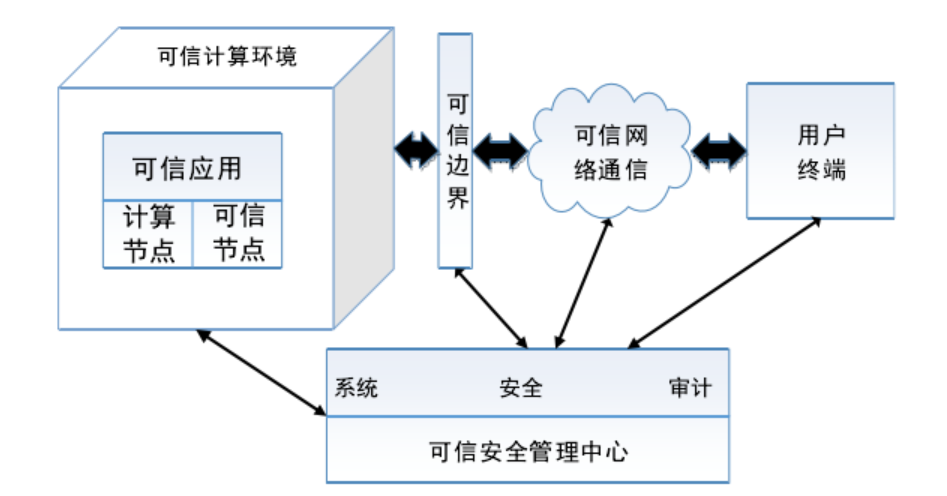
\includegraphics [width=0.5\textwidth]{./image/tu3-3.png}
\bicaption[labelFigtu3-3]{图}{\centering 三重防护架构}{Fig.}{\centering Triple protection architecture}
\end{figure}

该框架能实施多层隔离和防护,以防止某薄弱环节影响整体安全,并有效防止外部攻击。通过该3重防护框架,可以实现:

1.“非授权者不能获取重要信息”“重点做好操作人员使用的终端防护,把住攻击发起的源头关,进行强制访问控制,将有效防止非法操作。”

2.“不能读懂窃取的保密信息”“对重要信息采取加密等手段进行保护,非法用户只能拿到重要信息的密文。”

3.“系统和信息不可篡改”“实行系统资源管理,进行可信验证,使配置、代码信息不被篡改,并能自动纠错,阻止木马、病毒等恶意软件的入侵。”

4“系统高可靠性”“将攻击信息流有效分解,提高系统的健壮性和弹性,通过可信验证发现隐患,并能自动恢复。”

5.“抗抵赖性”“系统严格审计,及时记录违规操作信息,发现异常并进行跟踪,防止入侵者隐藏攻击痕迹。”

\subsection{智能电网安全架构模型研究}
\subsubsection{智能电网安全对象}
智能电网的安全对象指利用安全措施和安全架构,使得智能电网中各个系统的安全得以保证。智能电网中主要涉及到的系统包括智能信息系统,智能计量系统,数据交易系统,智能服务系统。

其中,智能计量系统指用户和电力传输中涉及到的系统,该系统负责管理调控用户用电计量,电力数据汇聚;电力传送中涉及到的电力分发,储存,还有记录如电流电压的参数等重要参数等;电力网格结构、配置等。

智能信息系统指从电力产生到用户消耗的每个环节中,各个环节都存在的一个负责监控,连接各环节,管理和配置,信息收集等功能的系统。该系统主要与智能计量系统交互,将确定好的配置传送给计量系统,从而让计量系统能够正确的计量,分发,储存电力等。

智能服务系统指智能电网中对用户提供服务的系统,包括查询,更改套餐等。该系统主要与智能信息系统交互,将用户选择的智能电网功能反馈给智能信息系统。

数据交易系统主要指在数据交易环节,涉及到数据买卖方,第三方使用的用户信息的交易,付费,管理系统。

\subsubsection{智能电网安全架构}
智能电网的安全架构是从智能电网需要涉及的安全技术角度进行描述。保证从建立安全的智能电网系统基础设施:包括计量设备,网关,传输线路,传输设备,分布式硬件。在安全的基础上,智能电网包括从顶至底,从硬件到软件都都存在的分布式体系,管理体系。具体实施环节中包含的用户侧、调度测的物理安全,计量系统安全,传输系统安全,信息收集安全。

\subsubsection{智能电网安全措施}

智能电网安全措施是以物联网安全措施的三重安全防护结构框架为基础,从智能电网的逻辑结构出发,在基础设施可信的环境下,对智能电网各个逻辑类的安全防护。基础设施指智能电网的可信基,包括:能源产生设备,电力消耗设备,连接系统。在具体的技术方面,要保证分布式控制系统可信,计量环境可信,信息系统可信,交易环境可信,就要做到:

1. 分布式控制系统

分布式控制系统是指位于调度侧的分散控制整个智能电网的各子系统,子模块的分布式调度管理系统。它承载了汇总,分析,计算,管理,查看,调度等所有重要功能。因此基本包含所有安全需求。分别有:人员方面要保证工作人员对其角色和职业的认知,做到合理的运维系统,并保证其专业知识是足够进行这种运维的;系统本身物理资产得到保护,同时具有实体访问控制能力,监督所有的进出,保证非授权人员无法访问机房;系统方面要有访问控制,身份认证功能,这些功能是为了保证非授权人员无法进入系统,接入系统的流程,设备的身份都是经过正确认证的;审计,问责要做到定期对系统日志,安全策略进行审计,保证其决策是正确的,并且这些决策在正确工作中;安全性评估是指系统需要具有监控和检测分布式控制系统的性能,保证其工作是可信的;风险管理评估是指对分布式系统中运用的所有技术和流程,运用它们可能涉及到的风险或暴露系统漏洞的可能性进行评估,要确保评估的完整性,持续性,以确保分布式控制系统的正确工作,从而确保其可信度;结构管理是由于智能电网中的分布式控制系统是需要经常进行策略或功能的添加,结构管理就是要确保这些新添加的结构是可信的。已经通过测试的;应急响应,备用方案是为了保证系统的持续工作性,要在系统发生突发事件如破坏性攻击时能够及时响应,或运用备用方案维持系统的工作,保证电力系统不会中断;日志与文档是指在分布式是控制系统中,功能的开发,改变,拷贝都是具有重大影响的,这些工作都需要在进行时进行日志和文档记录,而常规系统操作,数据访问等需要进行常规的查证,保证其操作是正确的,操作结束时保留的版本是正确的。

2. 计量环境可信

计量环境包含了调度侧和用户侧有关电力收集,计量,分发的环境。保证计量环境可信,需要做到计量设备物理安全;计量设备或系统访问控制功能,以防止非授权访问而产生的破坏数据;备用计量方案,以保证计量不会被中断从而遭受损失或错误;计量设备或系统需要具有配置管理功能,由于智能电网涉及到电力优化调度功能,因此计量环境的设置应具有可配置功能从而适应不用的电力方案,该方案在上线前也应是被充分测试后,证明是可行的;身份认证是指在数据计量,数据汇聚等计量环境中所有参与的计量设备应是正确的,而没有被破坏,添加等。

3. 信息系统可信

信息系统是智能电网中涉及用户管理,数据操作的系统。该系统与分布式控制系统的区别是信息系统主要控制管理智能电网中信息类数据类的功能,但信息系统的正常工作也是智能电网必不可少的一部分,同时因为人员参与控制信息系统,因此信息系统的安全需求与分布式控制系统基本类似,具体要求也与分布式控制系统类似,包括人员安全,人员专业知识训练,访问控制,安全监控评估,身份认证,配置管理,应急响应,备用方案,日志与文档管理,风险管理评估。

4. 交易系统可信

交易系统是用户信息交易的环境,包括交易者:买方,卖方,第三方,交易系统及交易管理系统。保证该系统可信主要确保交易中工作人员的合法身份,专业的、非违规的操作;对所有操作人员设有访问控制功能,保证非授权无法进行,保证操作人员无法使用非授权功能;利用日志和文档对所有数据操作,交易进行记录;并定期进行审计问责,保证交易的合规,在出现非授权交易时能够查询相应负责人员进行处理;具有结构管理功能,确保交易系统是可创建、可更新功能的。

\subsection{本章小结}
本章对物联网安全架构模型,智能电网安全架构模型的研究进行了详细的介绍。首先,本章介
绍了本文之前的在物联网安全方面的工作即物联网安全参考模型的研究。之后
结合目前实际情况将智能电网的结构与物联网安全参考模型的对象,架构,措施
三种元素结合,提出智能电网安全参考模型,并对模型中的每一个模块进行详细
的描述。

\section{基于异常检测的隐私安全技术研究}
\subsection{异常行为模式的定义}
本文定义的异常行为模式指的是用户隐私中尤其能表现与用户习惯反常的行为,通过描述对隐私的研究并与智能电网隐私结合来表明异常行为模式的定义和意义。

\subsubsection{用户隐私的定义}
目前并没有一个公认的,被国际通用的“隐私”定义,同时也没有相关法律法规对其进行明确定义,对不同的人来说定义都不相同。基本上,隐私可以当作是不被干涉的权利\citeBUAA{Warren1890Review}。并且,隐私概念经常与机密性,个人信息,机密信息等概念弄混,机密信息是应该是那些被限制的只允许应该接入的系统来访问的信息。而且,隐私也经常与安全混淆,其实两者有一部分是重复的,但是并不相同。我们认为用“保证安全可以不包括隐私安全,而要保证隐私安全必须确保安全”,也就说安全是隐私安全的一部分。传统安全是保密性,完整性,可用性。而隐私安全除了要确保保密性,完整性,可用性之外,还意味着隐私信息只按照最初的目的被收集,处理,使用一次\citeBUAA{CSW2010Privacy}。

那么在智能电网中,隐私就意味着用户的用电量,被收集用电量的权利,用户的利益等。Roger Clarke\citeBUAA{Clarke2006Workshop}对隐私分成的四个纬度很适用于智能电网的隐私概念,它们分别是:

1. 个人信息

这个维度是最常用的维度。个人信息包括个人涉及到的任何信息,这些信息可以直接的, 间接的标识出个人的身体,生理,精神,经济,位置,社会身份。并且个人拥有控制这些信息的权利,控制他们在任何时间地点方式被其他人访问的权利,并保证其不被泄露等。

2. 个人

个人是值个体能控制自己身体的完整性。包括身体条件,健康状况,医疗情况。

3. 个人行为

个人行为是个人能保证通过其活动,选择等而得到的知识被收集,使用,分享的权利。

4. 个人通信

个人通信指通信不被过度监督审查的权利。

\subsubsection{异常行为模式}
对应在智能电网中,第一个维度的概念完全适用,它意味着用户涉及到的用电信息,包括总用电量,用电时长,起止时间 (开关情况),每个电器用电量,每个电器用电时间等。并且智能电网硬件自动收集数据,用户应能控制这些数据的被收集,传输,挖掘的情况。第二三四维度的概念随着在智能电网对用电数据进行收集也产生。比如,由于用电数据带有时间戳,用户独特的对不同单独电器的使用习惯,与一般的用电习惯相比可以明显的表现出用户的用电习惯,用电行为。另外,如果家里使用电动车也能通过其充电情况表现用户出行习惯\citeBUAA{Clarke2006Workshop}。有一部分与之相关的工作是用电数据分解,利用隐马尔可夫模型或改进,通过总用电数据分解出每个电器的用电时间,用电量\citeBUAA{Kim2011Mining,Parson2012Types,Kolter2012Disaggergation},如图\ref{labelFigtu4-1}所示。这已经不只是第二三四维度的概念,第一维度的概念也被直接破坏。在第二三四维度中,对应到智能电网还有另一个问题,就是其他的参与方,实体或个人对数据的接入,如第三方。多方参与数据的收集与分析必然涉及到个人,个人通信的问题。首先在收集阶段,如果是硬件设备聚集数据还能有效保护数据,但如果数据汇集端刚在电力管理系统之类的应用中,由于软件安全,互联网安全而暴露的隐私问题就随之产生。
\begin{figure}[ht]
\centering
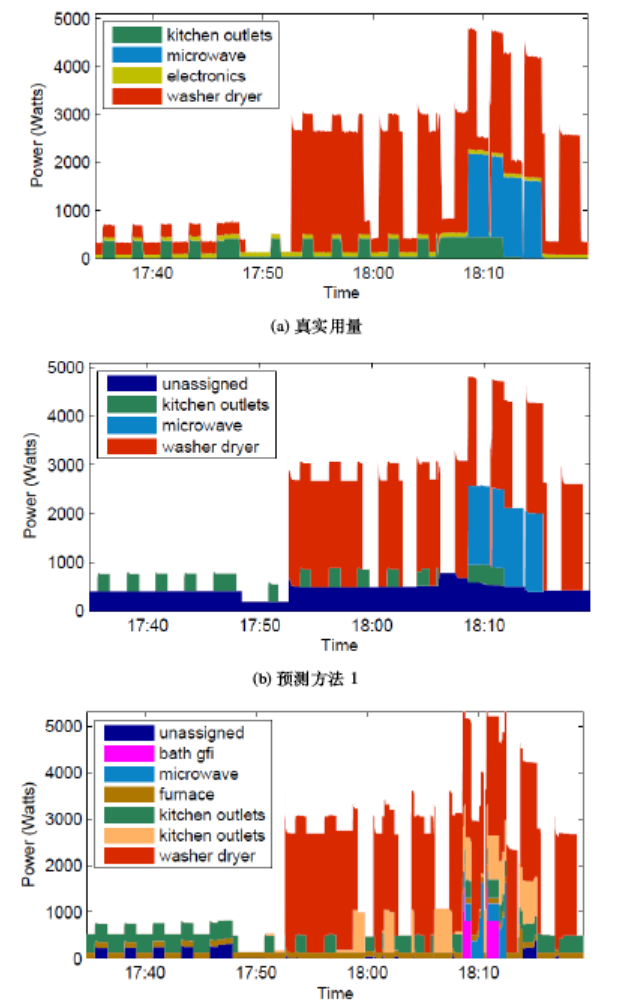
\includegraphics [width=0.5\textwidth]{./image/tu4-1.png}
\bicaption[labelFigtu4-1]{图}{\centering 用电数据分解}{Fig.}{\centering The disaggregation of usage}
\end{figure}

综上所述,我们认为智能电网隐私与传统隐私的主要区别在于智能电网信息反映用户行为习惯,包括用电起止时间,用电时长,带有时间戳的用量;还有多方参数的数据收集分析问题,包括第三方,数据提供者,数据购买者,攻击者等。

所以,我们认为将智能电网的隐私定义为传统的需要个体授权才能访问的信息是不够具体的,有意义的应该是智能电网中能够反映用户行为习惯的信息,并且这些信息需要用户授权才能访问。在2.4中我们分析了异常点的意义,异常点就意味着用户非日常活动,我们的工作就是在所有这些代表日常活动的隐私信息中挖掘更具有代表性的,能表现异常行为模式的异常点, 我们称之为异常行为模式挖掘。接下来我们将描述基于熵差的异常行为模式挖掘算法。

\subsection{基于异常模式检测的数据挖掘算法}
本文采用了基于内在模式和外在模式的熵差的异常检测算法,该算法借鉴了关键字检测的思想。文本聚簇性的关键词检测方法的核心思想是认为关键字在空间分布的模式中,更容易互相吸引,按照聚簇的形式出现,一般性的词在空间分布中则均匀出现。这与异常行为模式不谋而合,日常的生活习惯在生活中均匀出现,而异常行为模式则在如某个夜晚,某个白天等集中的时间内聚集出现。文本中熵的概念是指文本分布特性熵越大,其不确定性就越高,反之,熵越低则不确定性越低。本文参考了我们之前基于熵差的关键词检测工作\citeBUAA{Yang2013Applications},提出智能电网异常行为模式挖掘,下面进行详细描述。聚集出现的簇和均匀分布的组在空间上存在明显的统计特性。我们将这种统计特性描述为内在模式和外在模式。内在模式指示了数据出现了聚簇出现的统计特性,外在模式指示了聚簇消失的统计特性。内外模式的差就很明显的表现了表现出了分布与平均分布不相同的数据。在智能电网中,为了将按时间戳划分的用电数据适用于文本的检测方法,首先要对用电数据进行量化。按时间戳划分的用电数据量化将每一家30天以秒为间隔的数据量化为$Q$个等级,得到用电量等级来描述用户用电数量。之后就可以通过计算内外模式的熵和熵差用以显示在空间分布中聚类特性来检测异常点。基于我们的假设,我们认为用电行为的发生是有规律的,出现较大偏差的点违反这种规律视为异常行为模式。整个流程分为以下几步:

1)数据量化

在$REDD$数据集中,电力数据为以秒为间隔的离散数据,我们将时间分布视为空间分布,为了计算熵差,首先对数据进行量化,将所有数据分为
$Q$个等级,得到新的基于空间分布的电力用量数据。基于以秒为间隔的数据可以转换为以分、小时为间隔的数据。

2)计算熵差

计算量化后数据的熵差。熵差值较小的数据为分布较为平均的点,按照我们的假设,这些点为日常行为模式。而熵差较大的数据为与日常行为模式差异较大的点,这些点为异常点。对应到用电数据中,某用电等级在空间分布中出现的位置为$x_i$。具体计算过程如下:设平均距离为$\mu$,内部熵和外部熵为:
\begin{equation}
\label{eqnLabelp4-1}
d^I = \lbrace d_i|d_i<\mu \rbrace
\end{equation}
\begin{equation}
\label{eqnLabelp4-2}
d^E = \lbrace d_i|d_i>\mu \rbrace
\end{equation}
\begin{equation}
\label{eqnLabelp4-3}
d_i = x_{i+1} - x_i
\end{equation}

计算同一等级用电量前后距离$d$,则该等级用电量的内部熵和外部熵分别为:

内部熵:
\begin{equation}
\label{eqnLabelp4-4}
H(d^I) = -\sum_{d \in d^I} P_d \log_{2}(P_d)
\end{equation}

其中$P_d$为$d$在$d^I$中发生的可能性。

外部熵:
\begin{equation}
\label{eqnLabelp4-5}
H(d^E) = -\sum_{d \in d^E} P_d \log_{2}(P_d)
\end{equation}

其中$P_d$为$d$在$d^E$中发生的可能性。

因此内部与外部的熵差为:
\begin{equation}
\label{eqnLabelp4-6}
ED^q(d) = (H(d^I))^q - (H(d^E))^q
\end{equation}

对于日常的、行为模式非异常的用电等级,则是平均均匀的分布在整个用电
数据中,因此,其分布遵循几何分布:
\begin{equation}
\label{eqnLabelp4-7}
P(d) = p(1-p)^{d-1}
\end{equation}

其中$p$为该用电等级在全集中出现的概率,对于服从几何分布的用电等级,其熵差为:
\begin{equation}
\label{eqnLabelp4-8}
ED^{q}_{geo}(d) = (H_{geo} (d^I))^q - (H_{geo} (d^E))^q
\end{equation}

而将均匀分布的用电等级衡量为内部和外部模型,会得到两个部分的熵,这与其均匀分布是相违背的,因为为了使得其得到恒定的熵,使用下公式:
\begin{equation}
\begin{aligned}
E&D^{q}_{geo}(d) = \frac{ED^q (d)}{\vert ED^{q}_{geo}(d)\vert} \\
&= (-\sum_{d\leqslant \frac{D}{m} }\frac{p(1-p)^{d-1}}{p^I} \log(\frac{p(1-p)^{d-1}}{p^I})) \\
&-(-\sum_{d>\frac{D}{m} }\frac{p(1-p)^{d-1}}{p^E} \log(\frac{p(1-p)^{d-1}}{p^E}))
\end{aligned}
\label{eqnLabelp4-9}
\end{equation}
之后计算熵差得到的以秒、分钟、小时为间隔的敏感点。三种划分的聚簇分布在同一区间,其中秒和分的作用是用以确定异常数据到某分某秒。如图\ref{labelFigtu4-2-1}、图\ref{labelFigtu4-2-2}和图\ref{labelFigtu4-2-3}所示:

表示在原数据集中如图\ref{labelFigtu4-3}所示:

\begin{figure}[htbp]
\centering
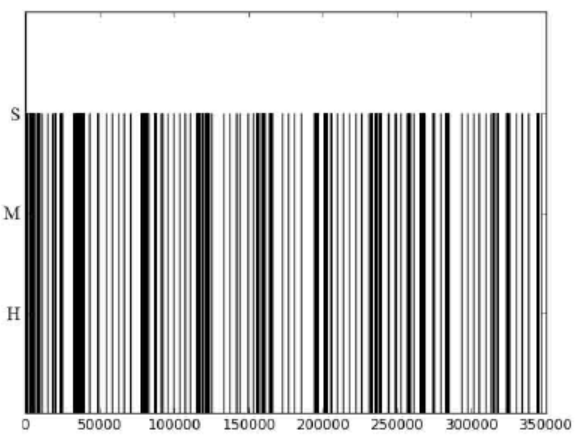
\includegraphics [width=0.5\textwidth]{./image/tu4-2-1.png}
\bicaption[labelFigtu4-2-1]{图}{\centering 异常用电数据位置-以秒为间隔}{Fig.}{\centering The position of usage outlier-In seconds interval}
\end{figure}

\begin{figure}[htbp]
\centering
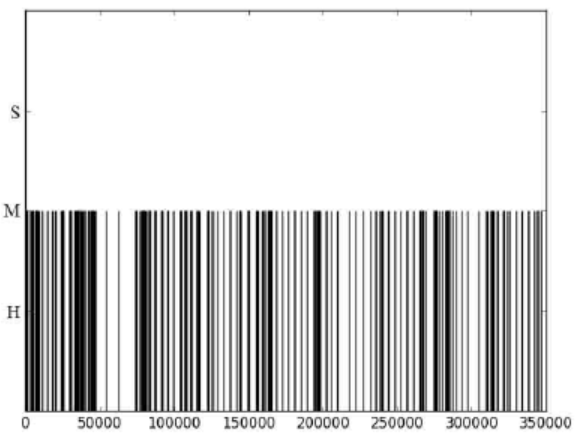
\includegraphics [width=0.5\textwidth]{./image/tu4-2-2.png}
\bicaption[labelFigtu4-2-2]{图}{\centering 异常用电数据位置-以分为间隔}{Fig.}{\centering The position of usage outlier-In minutes interval}
\end{figure}

\begin{figure}[htbp]
\centering
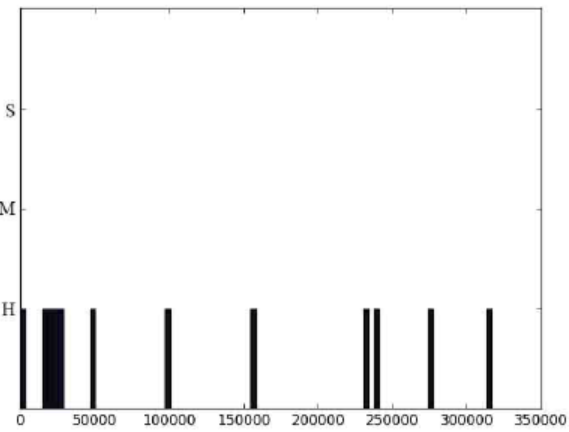
\includegraphics [width=0.5\textwidth]{./image/tu4-2-3.png}
\bicaption[labelFigtu4-2-3]{图}{\centering 异常用电数据位置-以时为间隔}{Fig.}{\centering The position of usage outlier-In hours interval}
\end{figure}

%\begin{figure}[htbp]
%\centering
%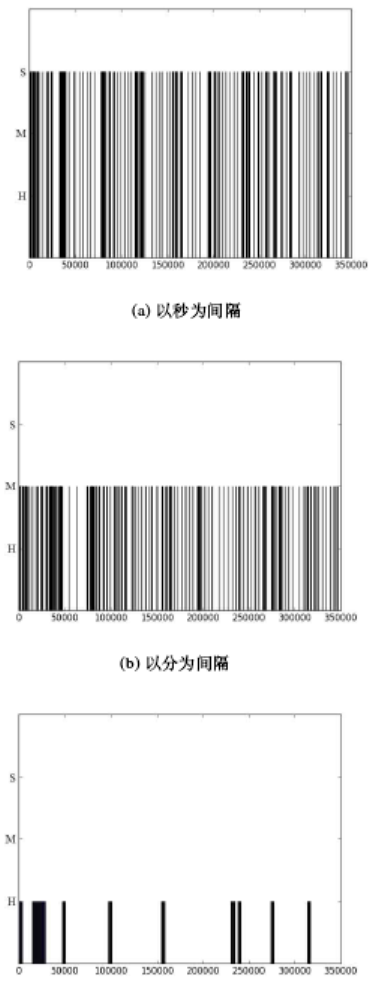
\includegraphics [width=0.5\textwidth]{./image/tu4-2.png}
%\bicaption[labelFigtu4-2]{图}{\centering 异常用电数据位置}{Fig.}{\centering The position of usage outlier}
%\end{figure}

\begin{figure}[htbp]
\centering
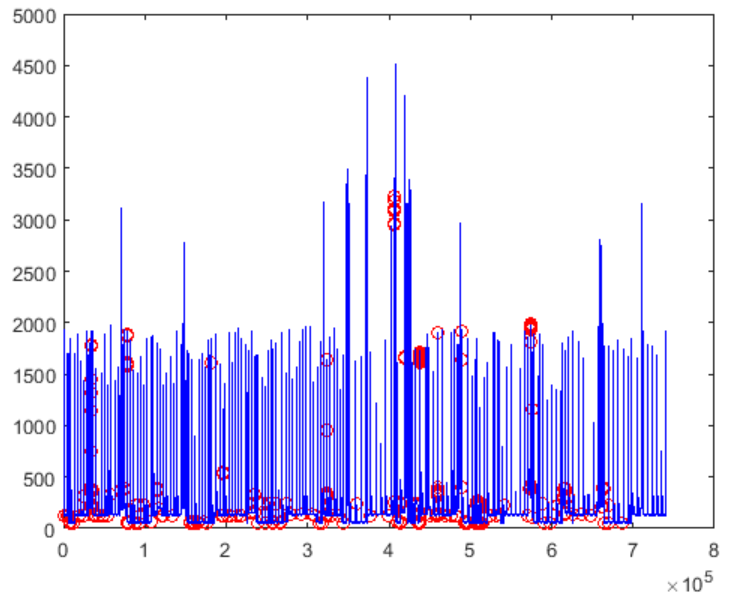
\includegraphics [width=0.5\textwidth]{./image/tu4-3.png}
\bicaption[labelFigtu4-3]{图}{\centering 异常点在原数据集中的位置}{Fig.}{\centering The position of outlier in source data}
\end{figure}

而不同用电等级熵差结果会产生自然排序,排序越前说明这个用电等级的行为模式越异常。

有一个问题要说明的是,在关键词检测时,可以通过关键字表或者人为判断是否是关键词,因此来选择排序中前$N$个词,但是隐私挖掘的工作是没有评判标准的,因此我们选择前26个熵差值大于0.01的量化等级,视其为异常点。如下表\ref{labelTabtab4-1}所示:

\begin{table}[htbp]
\centering
\captionnamefont{\xiaowuhao\bf }
\captiontitlefont{\xiaowuhao\bf }
\bicaption[labelTabtab4-1]{表}{异常行为排序}{Table}{Abnormal behavior rank}
\renewcommand\tabcolsep{1em}
% \xiaowuhao \selectfont
% \renewcommand{\arraystretch}{0.8}
% \fontsize{9}{11}\selectfont
\begin{tabular}{cccc}
\toprule
{排序} &  {量化等级} & {熵差}\\
\midrule
1 & 42 & 0.466131348\\
2 & 37 & 0.416908502\\
3 & 43 & 0.403831448\\
4 & 35 & 0.291582712\\
5 & 19 & 0.270527434\\
6 & 12 & 0.253194782\\
7 & 13 & 0.215926818\\
8 & 44 & 0.213194204\\
9 & 32 & 0.197048092\\
10 & 11 & 0.195808786\\
11 & 58 & 0.16018644\\
12 & 59 & 0.158423579\\
13 & 31 & 0.156878796\\
14 & 33 & 0.156878796\\
15 & 45 & 0.153834428\\
16 & 9 & 0.1525488\\
17 & 10 & 0.145075468\\
18 & 34 & 0.134315368\\
19 & 30 & 0.133014269\\
20 & 29 & 0.111050797\\
21 & 27 & 0.08343455\\
22 & 57 & 0.067384402\\
23 & 28 & 0.063893514\\
24 & 26 & 0.04672853\\
25 & 8 & 0.038229722\\
26 & 15 & 0.01208686\\
\bottomrule
\end{tabular}
\end{table}

\subsection{本章小结}
本章对用户隐私的概念,异常行为模式的意义,及异常行为模式挖掘方法进
行了详细的介绍。首先,对通用的隐私概念进行描述,并划分为四个维度。然后
针对这四个维度的隐私概念,描述智能电网中的隐私问题,及智能电网中异常点
的意义。最后,详细介绍了利用基于内在模式和外在模式的熵差法进行异常行为
模式挖掘的流程,公式及公式所表述的含义。

\section{实验设计}
\subsection{实验目标}
通过实验,我们希望我们能正确按照我们的定义挖掘出用户的隐私信息,并
评测这部分是否是合适的信息,具体如下:

基于熵差的异常行为检测效果如何?基于熵差的异常行为检测是基于位置
空间的检测法,将时间序列的电力数据视为空间数据。其本质是对空间位
置异常的检测,我们将本文的方法与几种经典的基于位置信息的检测算法
进行比较,利用评价指标验证效果。

\subsection{评估方法}
关于隐私信息挖掘没有公认统一的评测指标。我们选用相关工作中一个较
为直观且有意义的评价方法\citeBUAA{Ukil2014Workshops}。该方法设数据集为$S$,其中敏感数据部分设为$v$,非敏感数据部分为$\lambda$,则$S = v ∩ \lambda$。定义隐私测量指标为为测量隐私的难度,其实质意义是给出无标签数据集,在只知道$\lambda$的情况下,计算在数据集中测量到隐私的可能性,并用数值表示。这个概念与第二章中介绍的传统$PPDM$领域中的隐私量化不谋而合,本质上都是看攻击者通过原始数据能够寻找的信息量的大小。具体公式如下\ref{eqnLabelp6-1}所示:
\begin{equation}
\label{eqnLabelp6-1}
\Upsilon_{S,v} = \frac{\sum_{i=1}^{|v|}Pr(v_i)\log(\frac{1}{Pr(v_i)})}{\sum_{i=1}^{|S|}Pr(S_i)\log(\frac{1}{Pr(S_i)})}
\end{equation}

\subsection{实验设计}
为了验证本文提出的智能电网信息挖掘和隐私保护方法,实现我们的实验
目标,我们设计实验如下:

为了评价我们的位置信息检测方法的效果,与一般性的、基准性的工作进
行比较。因为数值上的挖掘工作一般是与标准差,改进的标准差等方法进
行比较,所以我们选择了基于空间的挖掘关键字的三种方法与我们的方法
对比。这三种方法是:标准差 $\sigma_{nor}$\citeBUAA{Carpena2009Squences},$Z-ScoreC$\citeBUAA{Carpena2009Squences}, 密度波动$\Gamma$\citeBUAA{Zhou2003Applications}。具体做
法是:分别利用这三种方法,对我们量化化好的电网数据等级进行异常点
挖掘,得到异常点排序,同样因为无法评测应该取得的阈值,我们将三种
方法按照取与我们之前的工作相同的阈值。四种方法分别利用上述评测方
法计算$\Upsilon_{S,v}$的数值,进行对比。

\subsection{本章小结}
本章我们对本文提出的提出的基于内在模式和外在模式熵差的异常行为检
测方法,设计两组实验,然后进行实验
验证及结论。通过本章我们与其他基本方法的对比说明我们的方法达到预期效
果,在有些不足的地方我们也进行了分析。

\section{结论}
物联网是科技发展到一定阶段的产物,物联网系统也将进入越来越多的行
业。作为国家重要能源系统的智能电网系统就是典型的物联网应用,但是智能
电网结构复杂,角色众多的特点决定智能电网一定会存在众多的安全问题,而
像智能电网系统这样的对国家,人民起到支撑性质的应用,一旦出现安全问题,
就会产生一系列严重的后果。因此,本文针对目前物联网结构及智能电网结构,
首先将智能电网分成安全对象,安全措施,安全架构,从措施和架构两个角度分
别阐述需要注意的安全问题,从而能够保证对象的安全。另外针对智能电网数
据能够反映用户日常生活习惯的隐私问题,提出了智能电网中的异常行为模式,
针对这种行为模式,提出基于熵差的异常行为挖掘方法,并提出智能电网数据隐
私保护方法。

首先,智能电网安全参考模型是基于物联网安全参考模型,将智能电网中
涉及到的所有硬件,软件,数据传输结构分解为物联网中的感知,传输,应用过
程,并根据智能电网的实际应用进行调整,感知对应智能电网中的计量环境,数
据传输对应智能电网中的信息系统和交易系统,应用则是安全对象。另外,智能
电网分布式的特性是由整体的分布式控制系统发起的,他连接汇总了智能电网
所有的组件,因此,安全措施是从智能电网的结构方面提出安全措施。安全架构
则是总结了智能电网各个组件涉及的所有安全问题,从需求的安全架构方面阐
述怎么才能保证智能电网组件的安全。

针对智能电网数据严重暴露隐私的问题,针对异常点这个问题,我们提出了
在智能电网中的异常行为的意义,并根据这个意义提出了基于熵差的异常行为
模式检测方法。该方法利用内在模式和外在模式的差异,检测一个序列中,分布
与正常均匀分布不相同的点,也就是在均匀的日常生活中,检测内在模式和外在
模式熵差较大的点,即与均匀的日常活动不相同的行为。

\vspace{1em}
{\hei\wuhao 致谢\quad}
{\fang\wuhao
感谢李琪老师悉心指导。
}



%%%%%%%%%%%%%%%%%%%%%%%%%%%%%%%%%%%%%%%%%%%%%%%%%%%%%%%%%%%%%%%%
%  参考文献
%%%%%%%%%%%%%%%%%%%%%%%%%%%%%%%%%%%%%%%%%%%%%%%%%%%%%%%%%%%%%%%%

\renewcommand\refname{\hei\wuhao\centerline{参考文献(References)}\global\def\refname{参考文献}}
\vskip 12pt

\let\OLDthebibliography\thebibliography
\renewcommand\thebibliography[1]{
  \OLDthebibliography{#1}
  \setlength{\parskip}{0pt}
  \setlength{\itemsep}{0pt plus 0.3ex}
}

{
\renewcommand{\baselinestretch}{0.9}
\liuhao
\bibliographystyle{unsrt}
\bibliography{./TempExample}
}



%%%%%%%%%%%%%%%%%%%%%%%%%%%%%%%%%%%%%%%%%%%%%%%%%%%%%%%%%%%%%%%%
% 作者简历
%%%%%%%%%%%%%%%%%%%%%%%%%%%%%%%%%%%%%%%%%%%%%%%%%%%%%%%%%%%%%%%%
{
\xiaowuhao
\noindent {\hei 作者简介:}

\noindent {\hei 程潇}~~~ 男,硕士研究生。专业:网络空间安全。
}

%%%%%!!!!!需要在合适位置插入\newpage,来平衡最后一页两栏!!!!!
% \newpage  %%% 用于平衡最后一页两栏高度

%%%%%%%%%%%%%%%%%%%%%%%%%%%%%%%%%%%%%%%%%%%%%%%%%%%%%%%%%%%%%%%
% % % 附录
%%%%%%%%%%%%%%%%%%%%%%%%%%%%%%%%%%%%%%%%%%%%%%%%%%%%%%%%%%%%%%%
%\vskip 20pt
%
% \noindent {\hei 附录A:}
%
%若确有特殊需要设附录的,附录部分置于作
%者简介后,标题为“附录A:”、“附录B:”......。公式
%用大写字母和数字顺序编号,例如“(A1)”, “(A2)”。




%%%%%%%%%%%%%%%%%%%%%%%%%%%%%%%%%%%%%%%%%%%%%%%%%%%%%%%%%%%%%%%%
%  英文摘要页
%%%%%%%%%%%%%%%%%%%%%%%%%%%%%%%%%%%%%%%%%%%%%%%%%%%%%%%%%%%%%%%%
%\clearpage
%\newpage
%% \cleardoublepage
%% \cleardoublepage\null
%% \newpage\null\thispagestyle{empty}\newpage
%\pagestyle{fancy}
%\fancyhf{}
%\lhead{}
%\chead{\vspace{0.8cm}\centering{{\CJKfamily{hei}\xiaowuhao 北\ 京\ 航\ 空\ 航\ 天\ 大\ 学\ 学\ 报}\\[-0.5ex]
%{{\xiaowuhao Journal of Beijing University of Aeronautics and Astronautics}}}}
%\rhead{}
%\lfoot{}
%\cfoot{}
%\rfoot{}
%\renewcommand{\headrule}{%
%\hrule height0.4pt width \headwidth \vskip1.0pt%
%\hrule height0.4pt width \headwidth \vskip-2pt}
%%%%%%%%%%%%%%%%%%%%%%%%%%%%%%%%%%%%%%%%%%%%%%%%%%%%%%%%%%%%%%%%%
%%          英文摘要
%%%%%%%%%%%%%%%%%%%%%%%%%%%%%%%%%%%%%%%%%%%%%%%%%%%%%%%%%%%%%%%%%
%
%\twocolumn[
%  \begin{@twocolumnfalse}\vspace*{0.3cm}
%\begin{center}
%\parbox{\textwidth}{
%\setlength{\parindent}{1em}
%{
%\centering\sihao\textbf{Title title title title title title} \xiaowuhao\fang (不超过10个实词,不出现非公知公用的缩写词)\\
%} \vspace{-1.2mm}
%\begin{center}
%{\wuhao ZHANG Moumou\makebox{$^{\text{1,2}}$}, LI Mou\makebox{$^{\text{1,2,*}}$}, SHANGGUAN Moumou\makebox{$^{\text{2,3}}$}, LIN Mou\makebox{$^{\text{3}}$}, ZHAO Mou\makebox{$^{\text{3}}$}, WANG Mou\makebox{$^{\text{3}}$}}\\[-0.1cm]
%\liuhao{(1. School of Aeronautic Science and Engineering, Beijing University of Aeronautics and Astronautics, Beijing 100191, China;\\
%2. School of Astronautics, Beijing University of Aeronautics and Astronautics, Beijing 100191, China;\\
%3. College of Automation, Northwestern Polytechnical University, Xi’an 710072, China)}
%\end{center}
%
%\vspace{-10pt}\wuhao
%{
%\textbf{Abstract:}
%(与中文摘要内容对应,英文摘要字数150\textasciitilde 200个单词)英文摘要应和中文摘要对应,并请导师
%或专业人士把关,保证摘要质量,高质量的摘要有利于文摘被国际权威数据库收录,及引起同行的重视。
%如果英文摘要比中文摘要更详细,应另提供一份英文摘要的中文副本,以便于本刊英文编辑检查英文。
%首次出现英文缩写时应注意写明全称。
%
%英文摘要的撰写规范请参考本刊网站“下载园地”中的《Ei文摘要求》。
%
%\textbf{Key words:} keyword1; keyword2; keyword3; keyword4; keyword5(与中文关键词一一对应,关键词请尽量从EI Controlled term中选择,以提高 EI检索的命中率及被引频次,网址:http://www.engineeringvillage.com/search/quick.url)。
%}
%}
%\end{center}
%
%%%%%%!!!!!英文脚注!!!!!
%\positiontextbox{2.0cm}{16cm}{
%\noindent\rule{4cm}{.5pt}\\[0.5ex]%
%\hspace*{1em} \xiaowuhao \linespread{0.8}\selectfont
%\parbox{\textwidth}{%
%\CalibriFont
%\hei\makebox[\widthof{\makebox{*}\textbf{R}}][r]{\textbf{R}}\textbf{eceived:} 2017-xx-xx; \textbf{Accepted:} 2017-xx-xx; \textbf{Published online:} 2017-xx-xx xx:xx\\%
%\hei\makebox[\widthof{\makebox{*}\textbf{U}}][r]{\textbf{U}}\textbf{RL:} \\
%\hei\makebox[\widthof{\makebox{*}\textbf{F}}][r]{\textbf{F}}\textbf{oundation item:} National Natural Science Foundation of China (12345678); China Postdoctoral Science Foundation(87654321)\\
%\hspace*{2em}(注:基金项目英文名称查询“基金项目的中英文名称”) \\
%\hei\makebox[\widthof{\makebox{*}\textbf{C}}][r]{\makebox{*}\textbf{C}}\textbf{orresponding author.} Tel.: 010-8231xxxx ~~ E-mail: bhxb@buaa.edu.cn
%}}
%  \end{@twocolumnfalse}
%]

%%%%%%%%%%%%%%%%%%%%%%%%%%%%%%%%%%%%%%%%%%%%%%%%%%%%%%%%%%%%%%%%
%  英文摘要页 结束
%%%%%%%%%%%%%%%%%%%%%%%%%%%%%%%%%%%%%%%%%%%%%%%%%%%%%%%%%%%%%%%%

\end{document}
